% This template was provided by Dr. Charles Welch
% He uses it in his course
%

\documentclass[11pt]{article}

% Change "review" to "final" to generate the final (sometimes called camera-ready) version.
% Change to "preprint" to generate a non-anonymous version with page numbers.
\usepackage[]{acl}
\usepackage{times}
\usepackage{latexsym}
\usepackage{natbib}

% For proper rendering and hyphenation of words containing Latin characters (including in bib files)
\usepackage[T1]{fontenc}
% For Vietnamese characters
% \usepackage[T5]{fontenc}
% See https://www.latex-project.org/help/documentation/encguide.pdf for other character sets

% This assumes your files are encoded as UTF8
\usepackage[utf8]{inputenc}
\usepackage{microtype}
\usepackage{inconsolata}
\usepackage{graphicx}

% If the title and author information does not fit in the area allocated, uncomment the following
%
%\setlength\titlebox{<dim>}
%
% and set <dim> to something 5cm or larger.

\title{ML Report:\\ VoiceBridge}


\author{Rawan Mahdi, Luna Aljammal \texttt{\{mahdir3, aljammal\}@mcmaster.ca}}

%\author{
%  \textbf{First Author\textsuperscript{1}},
%  \textbf{Second Author\textsuperscript{1,2}},
%  \textbf{Third T. Author\textsuperscript{1}},
%  \textbf{Fourth Author\textsuperscript{1}},
%\\
%  \textbf{Fifth Author\textsuperscript{1,2}},
%  \textbf{Sixth Author\textsuperscript{1}},
%  \textbf{Seventh Author\textsuperscript{1}},
%  \textbf{Eighth Author \textsuperscript{1,2,3,4}},
%\\
%  \textbf{Ninth Author\textsuperscript{1}},
%  \textbf{Tenth Author\textsuperscript{1}},
%  \textbf{Eleventh E. Author\textsuperscript{1,2,3,4,5}},
%  \textbf{Twelfth Author\textsuperscript{1}},
%\\
%  \textbf{Thirteenth Author\textsuperscript{3}},
%  \textbf{Fourteenth F. Author\textsuperscript{2,4}},
%  \textbf{Fifteenth Author\textsuperscript{1}},
%  \textbf{Sixteenth Author\textsuperscript{1}},
%\\
%  \textbf{Seventeenth S. Author\textsuperscript{4,5}},
%  \textbf{Eighteenth Author\textsuperscript{3,4}},
%  \textbf{Nineteenth N. Author\textsuperscript{2,5}},
%  \textbf{Twentieth Author\textsuperscript{1}}
%\\
%\\
%  \textsuperscript{1}Affiliation 1,
%  \textsuperscript{2}Affiliation 2,
%  \textsuperscript{3}Affiliation 3,
%  \textsuperscript{4}Affiliation 4,
%  \textsuperscript{5}Affiliation 5
%\\
%  \small{
%    \textbf{Correspondence:} \href{mailto:email@domain}{email@domain}
%  }
%}

\begin{document}
\maketitle
\begin{abstract}
Individuals with speech impairments resulting from neurological conditions, such as Parkinson’s disease, stroke, or cerebral palsy, face significant barriers when interacting with modern digital ecosystems. While flagship Automatic Speech Recognition (ASR) models have achieved high benchmarks for typical speech, their performance degrades sharply when processing dysarthric or atypical vocal patterns, limiting user independence. This paper presents VoiceBridge, an assistive software solution designed to bridge this accessibility gap.
\end{abstract}


\section{Introduction}

The VoiceBridge project addresses the digital accessibility gap faced by individuals with speech impairments resulting from neurological conditions like Parkinson’s disease, stroke, or cerebral palsy. While modern Automatic Speech Recognition (ASR) models have advanced significantly, flagship architectures such as Whisper and wav2vec often exhibit drastically reduced performance when processing atypical or dysarthric speech. This creates significant barriers to independence, preventing users from performing everyday digital tasks like messaging or browsing the internet. The goal of this initiative is to bridge this gap by fine-tuning a machine learning model to reliably interpret impaired speech and map it to actionable digital commands.

The system's objective is to capture impaired audio through a standard microphone and process it via a custom-trained machine learning model. The resulting text output is not merely for transcription but is designed to be mapped into actionable commands. By transforming these inputs into device-level controls—such as sending messages or operating applications—VoiceBridge aims to restore autonomy to users in everyday environments, including homes and clinics. This objective heightens the need for an accurate model to provide transcripts, as commands are often only a couple words in length. Due to the lack of context available to the model when processing short phrases, high recognition accuracy and low word error rate (WER) are vital for the systems relying on these model's performance.
\section{Related Work}

A semi-systematic review of ASR approaches for impaired speech indicates that fine-tuning large, pre-trained foundation models consistently outperforms models trained solely on typical speech \citep{voicebridge_litreview}. Research suggests that while full fine-tuning of all model layers can reduce WER by 30–60\%, it is computationally expensive and prone to overfitting when data is scarce \citep{voicebridge_litreview}. Consequently, parameter-efficient adaptation methods, such as Low-Rank Adaptation (LoRA) and adapters, have emerged as practical alternatives. As noted by \citet{pokel2025variational}, LoRA provides a reported WER reduction of 7–40\% while significantly lowering the computational load, making it suitable for deployment on standard hardware. Model families like Whisper are particularly attractive due to their out-of-the-box robustness and strong community support for fine-tuning on specialized datasets like UASpeech and TORGO.

Beyond model architecture, the literature emphasizes that preprocessing and feature engineering are critical for handling the irregular articulation and non-stationary noise often found in impaired speech recordings \citep{voicebridge_litreview}. Essential techniques include:

\begin{itemize}
\item \textbf{Temporal Normalization:} Methods such as Dynamic Time Warping (DTW) and Temporal Structure Normalization (TSN) address timing irregularities in dysarthric speech \citep{normalization_wav2vec}.
\item \textbf{Denoising:} DFT-domain subspace decomposition helps separate speech from background noise in uncontrolled environments \citep{sciencedirect_dysarthric}.
\item \textbf{Phoneme-aware Modeling:} Extracting phonetic representations (e.g., via Wav2Vec2-Phoneme) improves the precision of short command-based interactions \citep{huggingface_wav2vec2}.
\end{itemize}

\section{Dataset}

Training and evaluation data are drawn from the Speech Accessibility Project (SAP), a large-scale corpus of atypical speech collected to support ASR research for individuals with dysarthria and related conditions. SAP is well-suited to this work because it captures the acoustic characteristics, such as breathiness, irregular timing, and strained phonation, which cause performance degradation in general-purpose speech recognition systems.

A subset of 400 labeled utterances was used for fine-tuning, with an 80/20 train/validation split (320 and 80 samples respectively). A fully disjoint held-out set was reserved for evaluation; each utterance is paired with a ground-truth transcript and structured ratings covering the speaker's diagnosed condition and symptom severity across multiple dimensions. Training was conducted on SHARCNET H100 GPUs. As shown in Figure~\ref{fig:dataset-composition}, the subset is dominated by Parkinson's Disease (59.4\%) and ALS (26.1\%), with Cerebral Palsy (10.1\%), Down Syndrome (2.6\%), and Ataxic Dysarthria (1.8\%) providing coverage of acoustically distinct profiles.

\begin{figure}[t]
  \centering
  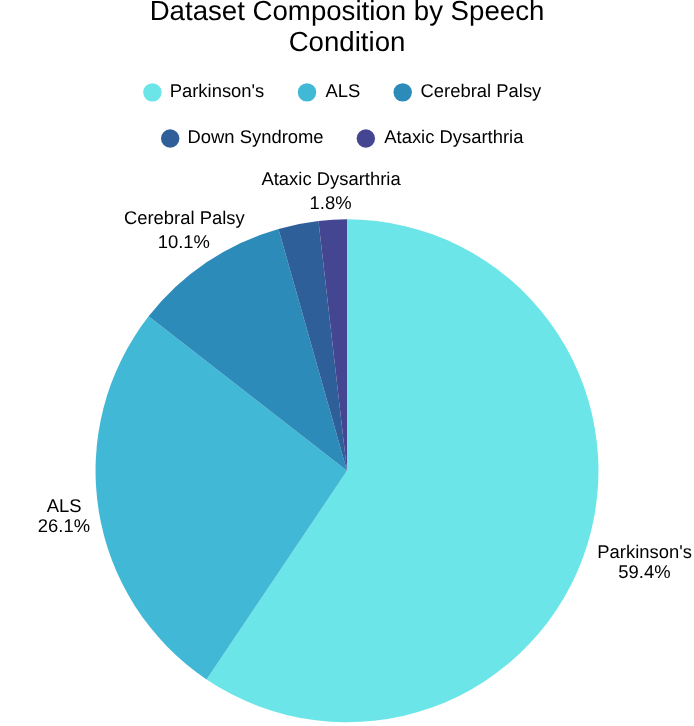
\includegraphics[width=\columnwidth]{figures/dataset-composition.png}
  \caption{Condition distribution of the SAP training subset.}
  \label{fig:dataset-composition}
\end{figure}

\section{Features}

The input representation follows the standard Whisper preprocessing pipeline: all audio is resampled to 16\,kHz and converted to log-Mel spectrograms via \texttt{WhisperProcessor}. 
Domain adaptation is achieved through Low-Rank Adaptation (LoRA), which augments the frozen pretrained model with trainable low-rank matrices injected into the attention layers. Rather than modifying the base weights, LoRA allows the model to acquire task-specific adjustments within a compact parameter space, learning the acoustic characteristics of dysarthric and command-style speech. Adapters are applied to the query and value projection matrices (\texttt{q\_proj}, \texttt{v\_proj}); training configuration and hyperparameters are detailed in Section~\ref{sec:implementation}.


\section{Implementation}
\label{sec:implementation}


The VoiceBridge implementation focuses on a parameter-efficient fine-tuning pipeline using Whisper-small as the foundation. 

\subsection{Data Preparation and Preprocessing}
The system processes audio samples standardized to a sampling rate of 16,000 Hz. A custom \texttt{AudioTextDataset} class manages the data pipeline:

\begin{itemize}
    \item \textbf{Audio Standardization:} Stereo signals are converted to mono by averaging channels to ensure consistency across different recording hardware.
    \item \textbf{Feature Extraction:} The \texttt{WhisperProcessor} extracts spectral features from the waveforms, while the associated tokenizer processes transcripts into input IDs.
    \item \textbf{Batching:} A \texttt{DataCollatorSpeechSeq2SeqWithPadding} handles dynamic padding for both input features and labels. Padding in labels is masked with a value of -100 to ensure it does not contribute to the loss calculation during training.
\end{itemize}

\subsection{Fine-Tuning with Low-Rank Adaptation (LoRA)}
To adapt the model to atypical speech patterns without retraining all 244 million parameters, the project utilizes the \texttt{peft} library to implement LoRA.

\begin{itemize}
    \item \textbf{Target Modules:} Adapters are applied specifically to the Query (\texttt{q\_proj}) and Value (\texttt{v\_proj}) projection matrices within the transformer's attention mechanism \citep{pokel2025variational}.
    \item \textbf{Hyperparameters:}
    \begin{itemize}
        \item \textbf{Rank ($r$):} Set to 16, providing a balance between model capacity and efficiency.
        \item \textbf{Alpha ($\alpha$):} Set to 32 as a scaling factor for the low-rank updates.
        \item \textbf{Dropout:} A rate of 0.1 is applied to the LoRA layers to prevent overfitting on the relatively small impaired speech datasets.
    \end{itemize}
    \item \textbf{Architecture Patching:} A \texttt{patched\_forward} method is used to wrap the base model, ensuring that the \texttt{peft} model correctly handles \texttt{input\_features} during the training pass.
\end{itemize}

\subsection{Training Configuration}
Training is conducted over 3 epochs using the \texttt{AdamW} optimizer.

\begin{itemize}
    \item \textbf{Learning Rate:} A stable rate of $1 \times 10^{-4}$ is maintained.
    \item \textbf{Checkpointing:} The system saves the model state dict to a \texttt{./checkpoints} directory every 100 batches, facilitating recovery and performance tracking across the training lifecycle.
    \item \textbf{Batch Size:} A batch size of 4 is utilized to fit within the memory constraints of standard GPU environments.
\end{itemize}

\section{Results and Evaluation}

Transcription quality is measured using Word Error Rate (WER), defined as
\[
  \mathrm{WER} = \frac{S + D + I}{N},
\]
where $S$, $D$, and $I$ denote substitutions, deletions, and insertions, and $N$ is the reference word count. For short commands, WER is a particularly consequential metric: a single error on a one- or two-word utterance constitutes a complete transcription failure and prevents command execution. All predictions and references are lowercased prior to scoring.

\paragraph{Baseline vs.\ fine-tuned.}
An unmodified \texttt{openai/whisper-small} model serves as the baseline. Both models are evaluated on the same 52-sample held-out set under identical decoding conditions. The baseline achieves an average WER of 0.813; the LoRA-adapted model reduces this to 0.558, an absolute reduction of 0.255 corresponding to approximately a 31\% relative improvement across the test conditions.

\paragraph{Per-condition analysis.}
Performance improvements are distributed across diagnostic groups but vary in magnitude. For Parkinson's Disease and ALS, fine-tuning substantially increases the proportion of near-zero WER samples and reduces high-error outliers. For Cerebral Palsy, WER decreases from approximately 0.75 to 0.45; for Ataxic Dysarthria, from approximately 0.65 to 0.35. Symptom-level analysis confirms that error distributions shift toward lower values across severity levels, indicating more consistent performance rather than selective gains on lower-severity speakers.



\section{Feedback and Plans}

The VoiceBridge project roadmap is strategically bifurcated into a \textbf{Minimum Viable Product (MVP)} and a set of \textbf{Stretch Goals} to ensure technical feasibility within the Capstone timeline while maintaining a path toward a comprehensive accessibility solution.
 
\subsection{Core Performance Benchmarks}
Success for the initial deployment is defined by two primary technical metrics:
\begin{itemize}
    \item \textbf{Transcription Accuracy:} A target of \textbf{70\%+ accuracy} on dysarthric speech. This represents a significant improvement over baseline Whisper-small performance for impaired speech.
    \item \textbf{Real-Time Latency:} Processing delay must remain \textbf{under 1 second}. This threshold is critical for interactive digital tasks, ensuring that the feedback loop between speech and device action feels natural and responsive for the user.
\end{itemize}

\subsection{User Experience and Feedback Loops}
To build user trust and mitigate the impact of ASR errors, the system incorporates a \textbf{non-disruptive feedback mechanism}. Transcribed text is displayed in a dedicated interface, allowing for immediate user verification. If a command is misinterpreted, the system provides clear pathways for manual correction, which not only assists the user but also provides potential data points for future iterative model refinement.

\subsection{Future Personalization and Environmental Robustness}
Expanding beyond the MVP, the team has identified several high-impact stretch goals:
\begin{itemize}
    \item \textbf{Custom Command Mapping:} Users will be able to define personalized "vocal shortcuts." For instance, a user with specific slurred phonemes can map a consistent distinct phrase to a high-level digital trigger, such as ``Open Browser'' or ``Emergency Alert''
    \item \textbf{Acoustic Robustness:} Current research focuses on enhancing ``Robustness to Noise'' \citep{sciencedirect_dysarthric}. This ensures the model remains functional in non-idealized environments, such as busy public clinics or domestic settings with ambient background noise.
\end{itemize}

\subsection{Project Timeline and Ethical Data Lifecycle}
The project is currently in the data collection and architectural refinement phase. 
\begin{itemize}
    \item \textbf{Phase 1 (Summer 2026):} Participant recruitment and audio data collection for fine-tuning will continue, coordinated with high-speed network support via ORION for large-scale data transfer.
    \item \textbf{Phase 2 (Fall 2026):} Detailed architectural reviews with technical advisors, including Pavel, will guide the final system integration and performance audit.
    \item \textbf{Phase 3 (Winter 2027):} The project is slated for official completion. In accordance with established ethics protocols, all raw research data will be permanently purged to protect participant privacy and comply with data retention agreements.
\end{itemize}

% \subsection{Tables and figures}

% % See Table~\ref{citation-guide} for an example of a table and its caption.
% % See Figure~\ref{fig:experiments} for an example of a figure and its caption.


% \begin{figure}[t]
%   \includegraphics[width=\columnwidth]{example-image-golden}
%   \caption{A figure with a caption that runs for more than one line.
%     Example image is usually available through the \texttt{mwe} package
%     without even mentioning it in the preamble.}
%   \label{fig:experiments}
% \end{figure}

% \begin{figure*}[t]
%   \includegraphics[width=0.48\linewidth]{example-image-a} \hfill
%   \includegraphics[width=0.48\linewidth]{example-image-b}
%   \caption {A minimal working example to demonstrate how to place
%     two images side-by-side.}
% \end{figure*}


% \subsection{Citations}

% \begin{table*}
%   \centering
%   \begin{tabular}{lll}
%     \hline
%     \textbf{Output}           & \textbf{natbib command} & \textbf{ACL only command} \\
%     \hline
%     \citep{Gusfield:97}       & \verb|\citep|           &                           \\
%     \citealp{Gusfield:97}     & \verb|\citealp|         &                           \\
%     \citet{Gusfield:97}       & \verb|\citet|           &                           \\
%     \citeyearpar{Gusfield:97} & \verb|\citeyearpar|     &                           \\
%     \citeposs{Gusfield:97}    &                         & \verb|\citeposs|          \\
%     \hline
%   \end{tabular}
%   \caption{\label{citation-guide}
%     Citation commands supported by the style file.
%   }
% \end{table*}

% Table~\ref{citation-guide} shows the syntax supported by the style files.
% We encourage you to use the natbib styles.
% You can use the command \verb|\citet| (cite in text) to get ``author (year)'' citations, like this citation to a paper by \citet{Gusfield:97}.
% You can use the command \verb|\citep| (cite in parentheses) to get ``(author, year)'' citations \citep{Gusfield:97}.
% You can use the command \verb|\citealp| (alternative cite without parentheses) to get ``author, year'' citations, which is useful for using citations within parentheses (e.g. \citealp{Gusfield:97}).

% \subsection{Equations}

% An example equation is shown below:
% \begin{equation}
%   \label{eq:example}
%   A = \pi r^2
% \end{equation}

% Labels for equation numbers, sections, subsections, figures and tables
% are all defined with the \verb|\label{label}| command and cross references
% to them are made with the \verb|\ref{label}| command.
% This an example cross-reference to Equation~\ref{eq:example}. You can also write equations inline, like this: $A=\pi r^2$.


% \section*{Limitations}

\section*{Team Contributions}
Rawan Mahdi Sections 1,2,5,7
Luna Aljammal: Sections 3,4,6

% Bibliography entries for the entire Anthology, followed by custom entries
%\bibliography{custom,anthology-overleaf-1,anthology-overleaf-2}

% Custom bibliography entries only
\bibliography{custom}

% \appendix

% \section{Example Appendix}
% \label{sec:appendix}

% This is an appendix.

\end{document}